\documentclass[
    %twocolumn
]{article}


% Packages
\usepackage[utf8]{inputenc} % For Norwegian letters
\usepackage{tabulary} % For nice tables
\usepackage{parskip} % For vertical spacing between paragraphs
\usepackage{float}
\usepackage{graphicx}
\usepackage{caption}
\usepackage{subcaption}
\usepackage[obeyspaces]{url}
\usepackage{listings}
\usepackage[margin=1in]{geometry}
\usepackage{wrapfig}

% Config
\graphicspath{{images/}}


\begin{document}

% Title
\title{\textbf{Exercise 3} \\ IT3708}
\author{Simon Borøy-Johnsen \\ MTDT}
\date{\today}
\maketitle
% End Title


% Content
\section{EA Parameters}
\subsection{Summarizing}
The EA parameters used for this system were quite similar to those used in the last exercise. In addition to the old parameters, the 20 best individuals from each generation spawned as children the next generation in order to implement a form of elitism. The parameters for this system can be seen in Table \ref{tab:parameters}.

The process of finding the parameters was exactly like the process used in the last exercise; I used the trial-and-error method, keeping in mind the parameters that worked well for the last exercise. I ran a lot of runs, varying different parameters (like population size, crossover- and mutation rates, selection functions), tracking the fitness curves, and comparing the results.

\begin{table}[H]
    \centering
    \begin{tabulary}{\textwidth}{|L|L|}
        \hline
        \textbf{Parameter name}         & \textbf{Parameter value} \\\hline
        Population size                 & 200 \\\hline
        Genome size                     & 1 bit for each connection ($=(6+1) * 3 = 21$). \\\hline
        Crossover probability           & 0.9 \\\hline
        Mutation probability            & 0.9 \\\hline
        Adult selection function        & Generational mixing \\\hline
        Parent selection function       & Tournament selection \\\hline
        Tournament selection group size & 50 \\\hline
        Tournament selection $\epsilon$ & 0.1 \\\hline
        Maximum number of generations   & 50 \\\hline
        Target fitness                  & 1.0 \\\hline
        Elitism number                  & 20 \\\hline
        Crossover method                & Splice genome \\\hline
        Mutation method                 & Genome-wise mutation \\\hline
    \end{tabulary}
    \caption{List of parameters used for the EA}
    \label{tab:parameters}
\end{table}

\subsection{Fitness function}
When implementing the fitness function, I tried making sure that the agent wouldn't become too biased towards neither eating all the fruit nor avoiding all the poison. By balancing the gain for eating as much food as possible against the penalty from eating poison, I was able to create a fitness function that provided good results. Equation \ref{eq:fitness_function} shows the maths behind the fitness function. The fitness is assessed by subtracting the proportion of all poison eaten from the proportion of all food eaten.

\begin{equation}
    fitness = \frac{\#eaten\ food}{\#total\ food} - \frac{\#eaten\ poison}{\#total\ poison}
    \label{eq:fitness_function}
\end{equation}

The equation makes sure that the agent wants to eat as much food as possible, whilst avoiding the poison. However, if the agent can acquire a higher score by eating some poison, it will do that. The optimal agent will eat all the food, and avoid all the poison, yielding a fitness of $1.0$. The worst possible fitness is achieved when eating all the poising and no food at all, yielding a fitness of $-1.0$.


\section{ANN Implementation}
\subsection{ANN design}

\begin{wrapfigure}{r}{0.5\textwidth}
  \begin{center}
    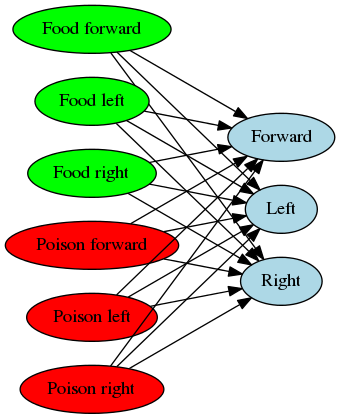
\includegraphics[width=0.48\textwidth]{network.png}
  \end{center}
  \caption{Design of the ANN}
  \label{fig:network}
\end{wrapfigure}

Figure \ref{fig:network} shows the final design of my ANN. The design is really simple, with no hidden layers. The input layer is fully connected to the output layer.

The input layer consists of six nodes, one for each input sensor (three food sensors and three poison sensors). The three output nodes represent the different moves the agent can make (except for the NOOP).

The activation function is the standard sigmoid function for all the nodes. The weights of the nodes are all binary, and the nodes' activation threshold is $0.5$.

\subsection{Design process}
In the beginning I set up the simplest network I could, with the same design as the final solution. The weights were binary, either the cell contained an element, or it did not. I set it up this way in order to be able to experiment with both the ANN design and EA design at the same time. Running the network with the same EA parameters as I used in the last exercise, (to my surprise) the network performed quite well.

I stopped focusing on the ANN design, and rather tweaked the parameters for my evolutionary algorithm. By tweaking the EA, I was able to get the final fitness values to about $0.80$ for both static and dynamic runs, with using both one and five different scenarios. At one point I tried adding a bias node for the output nodes, but this didn't yield any improvements in the performance.

As the classification issue in this exercise was fairly simple (mapping three sensor inputs to one of three different moves), the network didn't have to be complex at all. Based on the sensor input only, it should be really easy for the agent to make a rational decision. The mappings from inputs to outputs are very general; avoid poison, eat food, so the network should be able to solve the problem quite efficiently.


\section{Performance}
\subsection{Static run, one scenario}

\begin{wrapfigure}{r}{0.5\textwidth}
  \begin{center}
    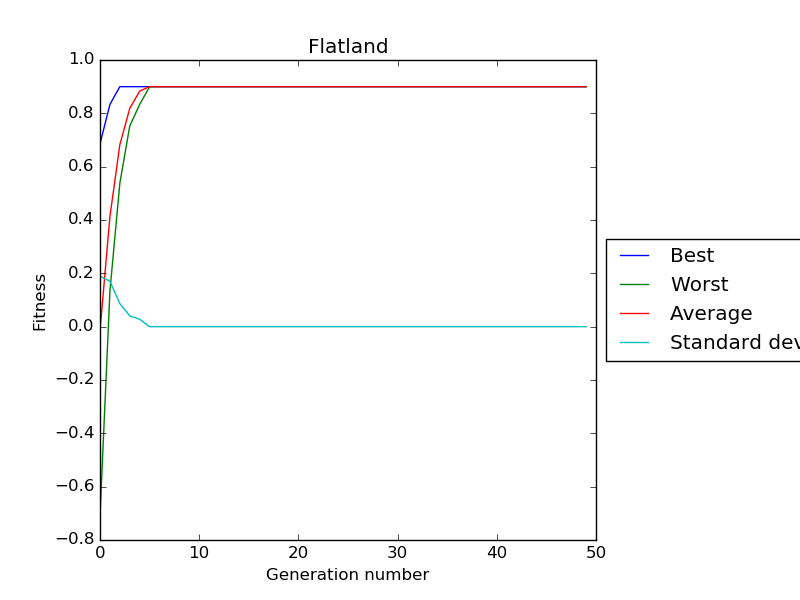
\includegraphics[width=0.48\textwidth]{static_one_static.png}
  \end{center}
  \caption{Fitness plot for the static run, using only one scenario}
  \label{fig:static_one}
\end{wrapfigure}

The best evolved agent was able to achieve a fitness score of $0.90$, eating $\frac{27}{30}$ food, and avoiding all poison pieces. The agent followed paths of food, while avoiding eating unnecessary poison. The three last pieces of food were hidden inside dangerous paths surrounded by a lot of poison, so the agent never dared going there.

When running the best evolved agent on a randomly-generated scenario, it performed just as well. The agent was able to achieve a fitness score of $0.89$, eating $\frac{30}{32}$ food, and only $\frac{1}{20}$ poison. The agent followed paths of food, while avoiding eating unnecessary poison. The one poison was eaten when the agent got trapped inside a poison "funnel", and the agent chose to eat its way out. The deduction of point from eating poison was lower than the gain from potentially eating the rest of the remaining food.

\subsection{Static run, five scenarios}

\begin{wrapfigure}{r}{0.5\textwidth}
  \begin{center}
    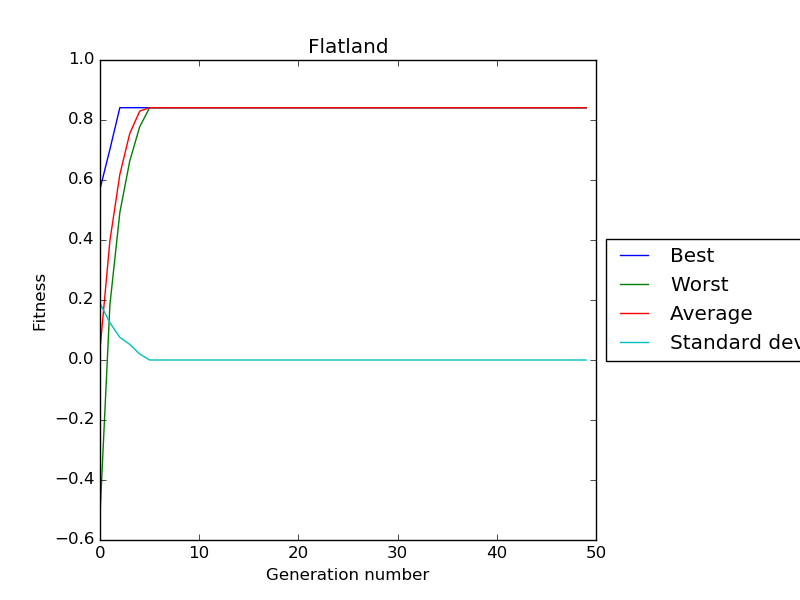
\includegraphics[width=0.48\textwidth]{static_five_static.png}
  \end{center}
  \caption{Fitness plot for the static run, using five scenarios}
  \label{fig:static_five}
\end{wrapfigure}

The best evolved agent performed about as well when training on five scenarios as when training on only scenario. The agent was able to achieve fitness scores of $0.97$, $0.90$, $0.81$, $0.67$, and $0.86$. The lower scores were achieved for the same reasons as for when only one scenario was used; getting stuck, or food pieces "hidden" behind poison pieces.

When running the agent on five randomly-generated scenarios, the scores varied a lot. This was most likely due to how badly the five scenarios used for training fitted the five scenarios used for testing.

\subsection{Dynamic run, one scenario}

\begin{wrapfigure}{r}{0.5\textwidth}
  \begin{center}
    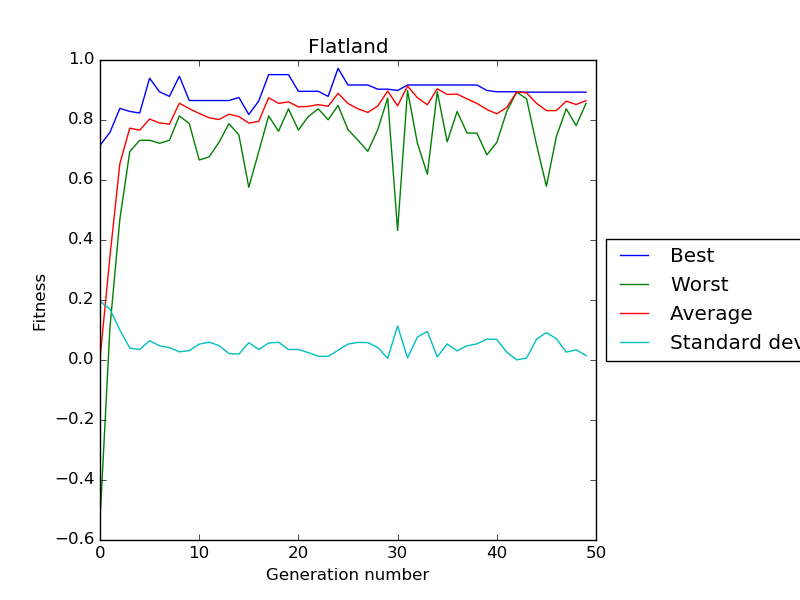
\includegraphics[width=0.48\textwidth]{dynamic_one.png}
  \end{center}
  \caption{Fitness plot for the dynamic run, using only one scenario}
  \label{fig:dynamic_one}
\end{wrapfigure}

For the dynamic run using one scenario, the fitness values oscillated a lot, as the agent's environment varied a lot. The selection pressure didn't get to apply in the same way as when training using static scenarios.

The best evolved agent achieved a fitness score of $0.77$, eating $\frac{30}{35}$ food, and only $\frac{2}{22}$ poison. Again, the behaviour was similar to that of the agent training with one static scenario.

\subsection{Dynamic run, five scenarios}

\begin{wrapfigure}{r}{0.5\textwidth}
  \begin{center}
    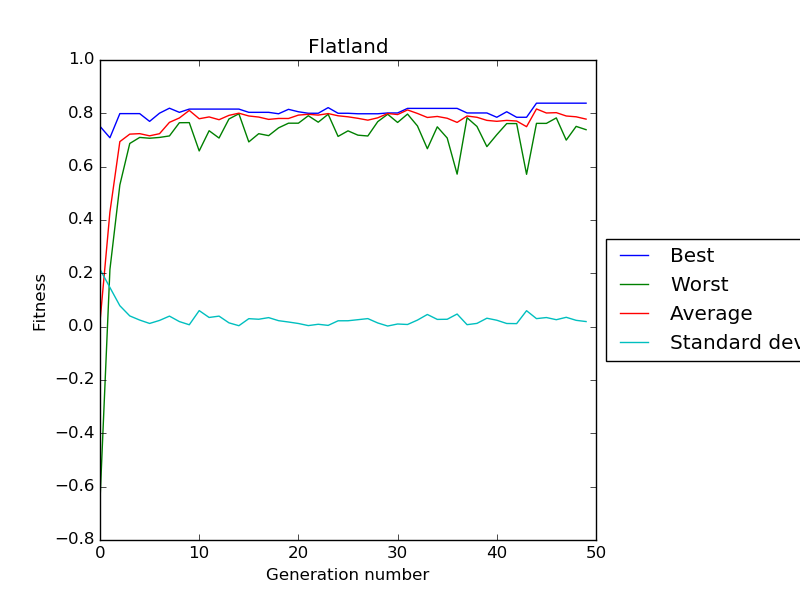
\includegraphics[width=0.48\textwidth]{dynamic_five.png}
  \end{center}
  \caption{Fitness plot for the dynamic run, using five scenarios}
  \label{fig:dynamic_five}
\end{wrapfigure}

Again, the fitness values oscillated, due to the same reasons as when using one dynamic scenario. But this time, the oscillations were not that big. The reason is that the five random scenarios are more general than a single scenario.

The best evolved agent performed slightly better when training on five scenarios as when training on only scenario. The agent was able to achieve fitness scores of $0.86$, $0.88$, $0.56$, $0.86$, and $0.78$. The lower scores were achieved for the same reasons as for when only one scenario was used; getting stuck, or food pieces "hidden" behind poison pieces.

\subsection{Difference in behaviour and plots}
The behaviour of the different agents didn't vary notably. All agents were able to make rational decisions, avoiding eating unnecessary poison, as well as eating the food they came across. This is due to the simplicity of the problem space. The difference in fitness scores are more likely to come from the generation of maps, as some maps simply are harder for the agents to perform well in.

The plots, however, varied a lot. For the static scenarios, the agents were quick to find near-optimal solutions. Therefore, the fitness values reached their maximum quite early. For the dynamic runs, the evolutionary algorithm was never able to find any generally good solution, resulting in oscillating fitness values.

% End content

\end{document}
